\documentclass[runningheads]{llncs}

\usepackage[utf8]{inputenc}
\usepackage[ngerman, english]{babel}

\usepackage[T1]{fontenc}
\usepackage{amssymb}
\setcounter{tocdepth}{3}
\usepackage{graphicx}
\usepackage{amsmath}
\usepackage{mathcomp}
\usepackage{url}
\usepackage[chapter]{algorithm}
\usepackage{algorithmic}
\usepackage{subfigure}

\usepackage{appendix}

\usepackage{listings}
\lstset{numbers=left, numberstyle=\tiny, numbersep=5pt}

\begin{document}
\mainmatter
\title{Trends and Concepts in the Software Industry II: \\ Development of Enterprise Software}
\author{Team 5: Providing Data Context During Development}
\institute{Thomas B\"unger, Felix Leupold, Johan Uhle, \\ Patrick Schilf, Lauritz Thamsen, Fabian Tschirschnitz \\[0.1in] Johannes Wust \\
Franziska Haeger, Dr. Anja Bog, Dr. Juergen M\"uller, Prof. Hasso Plattner \\
Hasso-Plattner Institute \\[0.1in]
March 15, 2013}
\date{March 15th, 2013}
\maketitle

\newpage

\tableofcontents
\newpage

%Head of Documentation - Patrick: gerade ziehen

\section{Introduction} 
%HoD
%Seminar, Seminarablauf, Thema (= deren how might we question)
%(dabei Bezug zu unserem Subthema aufbauen)
% close with an outline of this document, include references to all sections, see lables

%!TEX root = ../document.tex

\section[Design Thinking (Author: Felix Leupold)]{Design Thinking}
\label{sec:DESIGN_THINKING}

\emph{Design thinking} refers to the method of finding an innovative solution to an abstract or ill-defined problem. It attempts to structure the ideation process and provides guidelines, methodologies and frameworks that help in problem forming, -solving and -design. Design thinking is a human-centered approach with multidisciplinary collaboration and iterative improvements to produce innovative products, systems and services \cite{design_thinking_book}. There are various interpretations and definitions of design thinking. We refer to design thinking as defined by the Hasso Plattner Institue of Design at Stanford and Potsdam. In this definition the design thinking process contains six different phases, which are pictured in Figure \ref{fig:design_thinking_process}. The process is not linear, which is indicated by the connections amongst different non-succeeding phases. Every instance of a design thinking project is different. It is possible to jump back and forth between the different phases as you encounter new inflection points. 

%nochmal �berdenken
In the following, we briefly explain the aim of each phase as they also reflect the pathway in the course of our project and the structure of this report.

\begin{figure}
    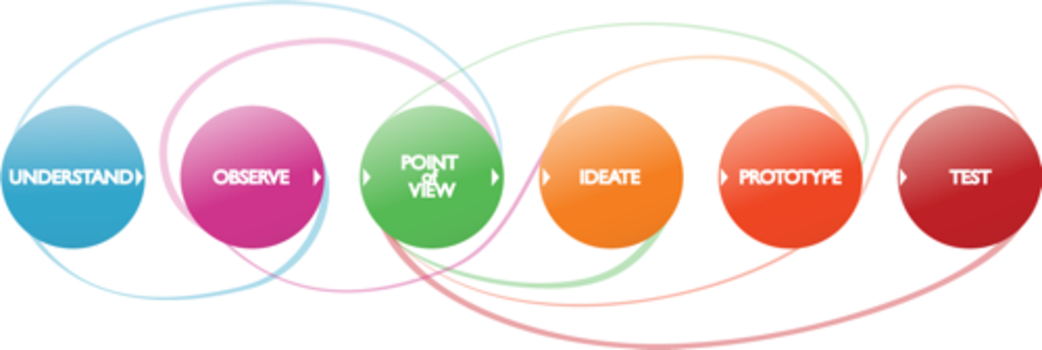
\includegraphics[width=\linewidth]{images/design_thinking_process}
    \caption{Design Thinking process according to \emph{Hasso Plattner Institue of Design} at Stanford and Potsdam.}
    % #selfrespect
    \label{fig:design_thinking_process}
\end{figure}

\paragraph{Understand}
In the first phase of the process, the team becomes familiar with the problem domain by talking to experts and conducting research. The goal is to develop background knowledge through these experiences. It is the foundation for all further steps. Throughout the process this stage might be visited again as new areas of problems, ideas or solutions emerge.

\paragraph{Observe}
What people say does not always correspond to their actual feelings, thoughts or actions. Therefore, it is necessary to watch how people behave and interact. These observations can be used to talk to users, ask questions and reflect on their behaviors. They lay the foundation for insights which are needed to define a point of view later in the process. Another point of this phase is to develop a kind of empathy for the user.

\paragraph{Point Of View}
The point of view consists of three parts: A persona, which is a concrete specification of the target user the team is designing for. Second, a need that this persona has and that the team is trying to satisfy with its solution. Lastly, an insight that has been generated from the observation made in the second phase. A commonly used method of defining a point of view is the "How might we..." question, which is a statement in a form "How might we help our persona to satisfy his or her need".
While the preceding phases tried to capture a wide range of users and problems, in this stage the team settles on a single point from which it can converge again in the next phase.

\paragraph{Ideate}
While the first three phases focus on defining and understanding the problem, the ideation phase opens up the solution space for the problem. The team is challenged to brainstorm as many solutions as possible by going for quantity, deferring judgment and building on the ideas of others.

\paragraph{Prototype}
Prototyping is a crucial part of the design thinking process. It allows to make the ideas visible and tangible. Quick and cheap prototypes, e.g. sketches on paper, are well suited for conveying the idea and getting feedback. People tend to hesitate to criticize or suggest changes for overly polished prototypes. A key concept is to fail early and often.

\paragraph{Test}
In the test phase the team collects feedback on their ideas which they made experienceable through their prototype. The goal of this phase is to learn which parts of the design work and which don't.
Testing ensures that the product is desirable for the end user and stresses the user focus of design thinking.
Latest from here on the team continues with one of the earlier phases.

\paragraph{}
Each potential solution has to satisfy three requirements as depicted in Figure \ref{fig:desire_viable_feasible}. Desirability ensures, it addresses an actual need of the user. Feasibility means that the solution should be technically possible to implement. Lastly, it has to be viable for the business partner providing the solution.
Innovative solutions lie in the intersection of the three sets. Design thinking helps to find solutions that lie in this intersection.

\begin{figure}[H]
\begin{centering}
    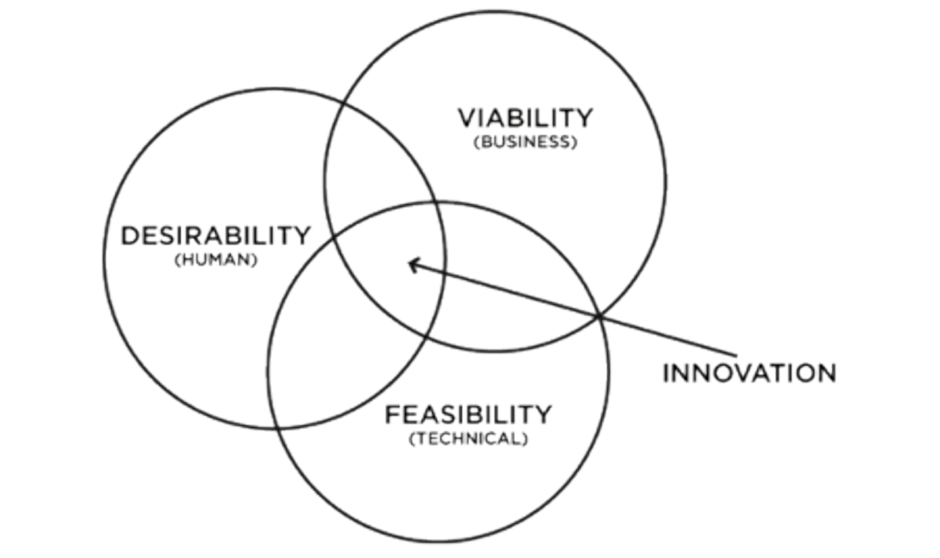
\includegraphics[width=0.5\linewidth]{images/desire_viable_feasible}
    \caption{Solution can be categorized into different sets. An innovative solution has to be viable, desirable and feasible.}
    % #selfrespect
    \label{fig:desire_viable_feasible}
\end{centering}
\end{figure}
%intro to Design Thinking, its cycle and some intro to our results 

\section{Understand} \label{sec:UNDERSTAND}
%Johan
%Pre seminar interviews

\section{Observe} \label{sec:OBSERVE}
%Johan
%Bachelor projects, conventional development (edit, build, compile)

%!TEX root = ../document.tex

\section[Point of View (Author: Felix Leupold)]{Point of View} \label{sec:POINT_OF_VIEW}

A point of view (POV) consists of three parts: a concrete specification of the user we are designing for, his or her needs we are trying to satisfy with our solution and finally an insight we derived from the understanding and observation phase. We present all of these in this section.

We derive a \emph{"How might we..."}-question from our POV and try to answer this question during the ideation phase. This description presents our final Persona and her needs. Throughout the course we repeatedly adapted our Persona slightly as we discovered new needs and reevaluated their importance for our persona.

\subsection{Persona}
\label{subsec:persona}

Our Persona is Amber, she is 31 years old and for roughly six years has she been working as a Software Developer at a big company that use HANA as a database for their applications. Within her team of ten developers, she programs applications that work on big data sets and are performance critical. While her main focus is on the backend side, she does not consider herself a database expert. Though she still knows how to write SQL queries, she is not able to predict the impact of certain changes in a query formulation on its performance just by looking at the statement. She works in her favorite development environment studio, which is Eclipse\footnote{\url{http://www.eclipse.org/}}. As a seperate environment, HANA Studio allows her to look at the content or schema of the database.

Amber enjoys coding a lot. It is the favorite part of her work. She is also very enthusiastic and wants to get features completed as fast as possible. She uses a lot of different tools that help her simplify reoccurring tasks and boost her productivity.

However, throughout her work day Amber usually experiences a lot of interruptions. We refer to these interruptions as \emph{Context Switches} that pull her out of her workflow. These might be small switches, like changing from the editor to the browser to browse for something online but can also be bigger ones, such as having to write an email or even physical interruptions caused by colleagues who ask for her attention.

\begin{figure}
    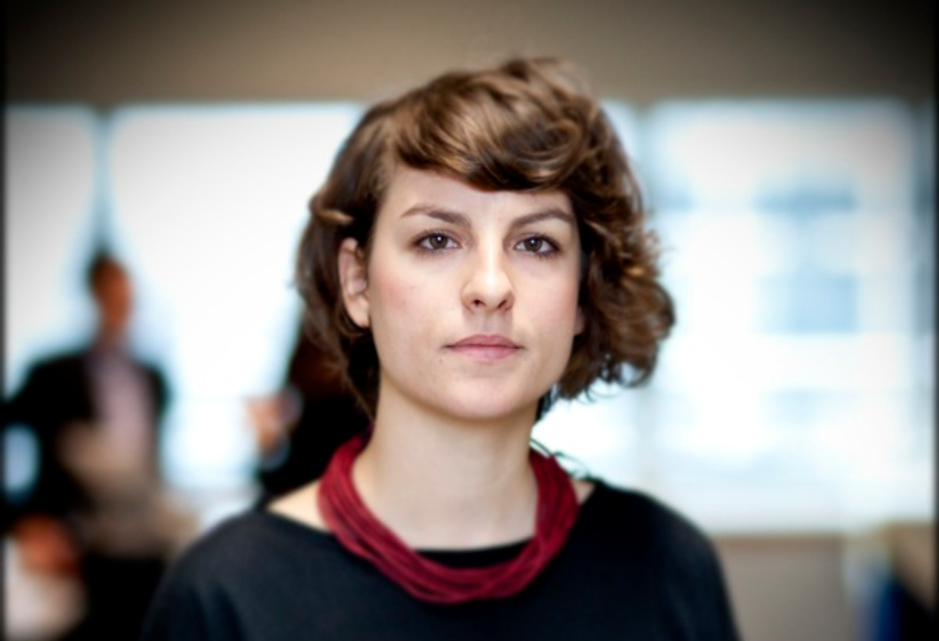
\includegraphics[width=\linewidth]{images/amber}
    \caption{Our Persona Amber, a software developer for performance critical big data applications.}
    % #selfrespect
    \label{fig:amber}
\end{figure}

\subsection{Needs}
Amber's needs are manyfold. The essential ones are:

\begin{itemize}
	\item She wants to do her work in the most efficient way.
	\item Since her applications are performance critical, she needs to evaluate her code against real customer data.
	\item Amber is not an SQL expert. Thus, she needs a way to explore and learn which parts of a query perform well and where bottlenecks are.
	\item She wants her productivity tool chain to be integrated into her IDE in order to avoid switching contexts.
	\item The general number of Context Switches needs to be minimized.
\end{itemize}

Throughout the seminar we down-weighted the importance of the last point as we narrowed down the interruptions that we wanted to tackle. We discovered that although big Context Switches like replying to emails lead to longer disruptions, they occur way less frequently than small Context Switches, such as navigating between applications. Thus tackling issues of the latter type may, accumulated, lead to a big increase in efficiency which is why we focused on that.

\subsection{Insight}

During our observations we saw how our Persona figured out to understand SQL queries written in code. She copied the query from her Eclipse editor into HANA Studio. As in Eclipse her query appears as multiple split \emph{Strings} she has to escape all contained quotes. This is the first Context Switch. Most queries also contain parameters that are bound during runtime. In order to execute the query in HANA Studio Amber looks up appropriate values in the schema. This is the second Context Switch. If the executed query does not behave as expected she is forced to go over this whole process again, switching back and forth in the Studio between edit- and result-view mode. There is no way to recognize the impact of query changes on the result in the same window. Thus, this results in a number of additional Context Switches. If the query finally behaves as desired, Amber has to copy it back into her code editor and turn all concrete values back into variables.

We consider this interaction as a workaround and take it as a foundation for our Point Of View as it emphasizes the most important need. That is predicting the impact of queries on the underlying data. We combine our Persona and her need with one of the insights we gathered during our interviews, namely that \textit{Code needs data context} (cf. Section \ref{sec:OBSERVE}).


\subsection{POV Statement}

\begin{description}
	\item [User] Amber, a productivity junkie, working with HANA on performance critical big data business applications.
	\item [Need] Amber needs to predict the performance and logical impact of her code on the underlying data sets using only without switching to another application.
	\item [Insight] Code needs data context.
\end{description}

Based on this, we derived the following \emph{"How might we question..."}:

\subsection{How Might We...}

\begin{quote}
\emph{"How might we help Amber to predict the impact of her code on real customer data in one integrated development environment?"}
\end{quote}
%Felix

\section{Ideation} \label{sec:IDEATION}
%Felix
%our idea, plus make up some ideas that were not followed

\section{Paper Prototype} \label{sec:PAPER_PROTOTYPE}
%Thomas

\section{User Testing and Feedback} \label{sec:USER_TESTING}
%Thomas
%Testing
%Feedback

\section{Final Prototype} \label{sec:FINAL_PROTOTYPE}
%Fabi

\section{Implementation Ideas} \label{sec:IMPLEMENTATION_IDEAS}
%Lauritz
\subsection{Gathering Data Contexts}
%tracing data contexts = snapshots of database and parameters and state, show code examples with parametrized queries
%from test systems with copies of real customer data or from actually deployed and running customer systems
\subsection{Selecting Data Contexts}
%developer always makes the final decision, has to be able to tweak any preselection and also to explore the full extent of gathered data contexts
%automatic sampling using clustering, include clustering image
%tweaking or explicit preselection by involved domain experts

\section{Open Questions} \label{sec:OPEN_QUESTIONS}
%Lauritz
\subsection{Hardware Context}
%runtime characteristics as, for example, query execution profiling depends on the hardware, hardware-aware data contexts, execution on actual hardwares or simulation of hardware, requires research, that is, hardware contexts are future work
\subsection{Query Debugging}
%besides seamless debugging of application-layer code and database-layer queries
%seeing results and profiling information not only for complete queries and distinct subqueries in from clauses, but also for partial queries, obviously not possible to execute arbitrary parts of queries, as, for example, the select query might depend on the presence of a grouping (show example query), therefore, support developers in identifying meaningful parts of queries to, for example, just activate a part of the conditions available in a given where clause, obviously also requires a user interface that allows to select and deselect potentially combinations of just parts of queries
\subsection{Efficient Context Storing}
%many traces result in many contexts, which might be similar, consequentely, identifying and, subsequentely, storing common bases along with context differences might reduce the memory consumption of a context database significantly, for the database snapshots it might be possible to leverage HANA's time travel feature

\section{Conclusion} \label{sec:CONCLUSION}
%HoD

\bibliography{references}
\bibstyle{splncs03}
\bibliographystyle{splncs03}

\end{document}
